%INSTALL Pygments sudo apt-get install python-pygments


\documentclass[letterpaper,twocolumn,10pt]{article}
\usepackage{usenix,epsfig,endnotes, upgreek, beamerarticle}
	\setbeamercovered{transparent}
\usepackage{listings}
\usepackage{pxfonts}
\usepackage{amsmath}
\usepackage{amssymb}
\usepackage{parskip}
\usepackage{color}
\definecolor{cool}{rgb}{0.5,0.2,0.5}
\usepackage{graphicx}
\newcommand{\code}[1]{\texttt{#1}}
\usepackage[noend,linesnumbered]{algorithm2e}
\begin{document}

%don't want date printed
\date{}

%make title bold and 14 pt font (Latex default is non-bold, 16 pt)
\title{\Large \bf CSE 231 Project 1}

\author{
{\rm Michael Barrow}\\
mbarrow@eng.ucsd.edu\\
University of California, San Diego
\and
{\rm Jules Testard}\\
jtestard@eng.ucsd.edu \\
University of California, San Diego
\and
{Konstantinos Zarifis} \\
zarifis@eng.ucsd.edu \\
University of California, San Diego
}

\maketitle

% Use the following at camera-ready time to suppress page numbers.
% Comment it out when you first submit the paper for review.
\thispagestyle{empty}

%\subsection*{Abstract}
%This report describes the implementation and experimental results of custom LLVM passes applied to supplied benchmark programs. The high level concept of each pass is discussed, followed by key implementation details. Finally we offer conjecture on experimental application of these passes. %This is the structure of the benchmark code is evaluated with respect to pass output 

\section{Introduction}
We present here an implementation of a data flow analysis module for the C++ LLVM compiler. Our implementation includes four types of analyses 1) Pointer Analysis 2) Constant Propagation 3) Available Expressions 4) Range analysis. All analyses are made on a function scope. We first present our interface followed by detailed description of the implementation of each analysis.

\section{Static instruction count}
%\textbf{Problem statement: } \textit{Write a pass that counts the number of static instructions in a program.} \\
%\textbf{Problem instance:} \textit{Output for each instruction the number of times it appears in the program.}
\subsection{Pass Algorithm description}

Because the functionality is a static analysis, it is sufficient to run a pass on the compiled code of each benchmark.
We store instruction op codes and their corresponding count in a C++ map structure. Each time an instruction is found in the source code, it is either added to an existing map entry or a new entry is created and initialized to 1.

A high level algorithm description is given on algorithm 1, where :
\begin{itemize}
\item {$I$ is an input program instruction list in LLVM byte code (.bc) format}
\item{$i$ is an individual instruction within $I$}
\item{$M$ is a C++ map of the form \code{<string,int>}}
\end{itemize}

\begin{algorithm}
 \KwIn{$M$,$I$}
 $t \gets 0$\\
 \ForAll{$i \in I$}
 { 
 	\If{$M$.containsKey($i$)}
 	{
 		$M$.valueForKey($i$)+=1\\
 	}
 	\Else
 	{
 		$M$.insertKeyValuePair($<i$,$1>$)\\
 	}
 }
 \ForAll{keyValuePair $\in M$}
 {
 	print("Found "keyValuePair.value() "counts of: "keyValuePair.key())\\
 	$t$ += keyValuePair.value()\\
 }
 print("total instructions: "$t$)
 \caption{Static instruction count algorithm}
\end{algorithm}

\subsection{Physical Implementation Description}
%Besides a working proficiency in C++, translating the algorithm to LLVM required an understanding of:
%\begin{itemize}
%\item how to build and run an opt module on a target benchmark program
%\item how to output data in human readable format from an opt module
%\item how instructions are represented by LLVM
%\item how instructions are accessed by opt modules
%\end{itemize}

While the above is the abstract description of what we are trying to achieve, we have to adapt our algorithms to the syntax and semantics of an LLVM \code{opt} pass framework. The general purpose of an \code{opt} pass is to instrument an input bitcode file and ouptut its instrumentation. This process is done using different C++ classes (and methods) depending on the scope of the instrumentation. We chose to use the \code{ModulePass} class (and \code{RunOnModule(Module \&M)} method) which gives us simultaneous access to all the functions in the input file, make are counting task easier. \\

In order to represent the $\textbf{forall the } i \in I$ iteration, we use the iterator abilities of the Module and Function classes as follows :

\begin{frame}[fragile]
%\frametitle{Inserting source code}
\lstset{language=C++,
                basicstyle=\ttfamily,
                keywordstyle=\color{blue}\ttfamily,
                stringstyle=\color{red}\ttfamily,
                commentstyle=\color{green}\ttfamily,
                morecomment=[l][\color{magenta}]{\#}
}
\begin{lstlisting}
for (Module::iterator m = M.begin(),
    e = M.end() ; e != m ; ++m) {
    for (inst_iterator I = 
    inst_begin(m), E = inst_end(m) ;
    I != E ; ++I) {...}
\end{lstlisting}
\end{frame}

The body of the algorithm (lines 3 to 6) could then be implemented using standard C++. Finally, to output the results of our analysis we implemented the \code{void print(raw\_ostream \&OS, const Module\*) const} function which allows use to print out our analysis result using the \code{-analyze} flag of the \code{opt} module. 

%\begin{frame}[fragile]
%\frametitle{Inserting source code}
%\lstset{language=C++,
%    basicstyle=\ttfamily,
%    keywordstyle=\bfseries,
%    showstringspaces=false,
%    morekeywords={runOnModule}                
%}
%\begin{lstlisting}
%    virtual bool runOnModule(Module &M)()
%\end{lstlisting}
%\end{frame}

%Accessing instructions was accomplished by iterating through the \textbf{input source} \textbf{Module} using an \textbf{inst\_iterator}. The Module contains all instructions from the compiled benchmark and the inst\_iterator points at individual instructions.\\


\subsection{Benchmark analysis}
We analysed module performance by comparing the logged instruction count with manual and automatic counts of the intermediate .ll byte code of each compiled benchmark. The automated counts were performed with the grep command
\code{cat [benchmark-name.ll] | grep [instruction-name] -c}. The counts were accurate, confirming the pass' correct functionality.
%\begin{figure}[here]
%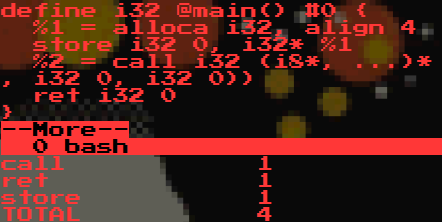
\includegraphics[width=0.4\textwidth]{StaticInst}
%\caption{Example correct pass output}
%\label{StaticInstCount}
%\end{figure}
\section{Dynamic instruction count}
%\textbf{Problem statement: } \texit{Write a pass that counts the number of times each instruction is used when a program is executed.} \\
%\textbf{Problem instance:}

\subsection{Pass Algorithm Description}
We want to write a pass which counts the number of times each instruction is used when a program is executed. We cannot do this by a simple static analysis of the program, we need to instrument its bitcode by adding instructions that will count each instruction in the initial program whenever it is used during the execution, while making sure the instructions we added are not counted themselves.

\begin{algorithm}[here]
%\SetKwFunction{count}{count}
%\SetKwFunction{print}{print}
\textbf{count}(Instructions $I_B$)  \Begin {
	\ForEach{$i \in I_B$}{
	 	\If{$M$.containsKey($i$)} {
 			$M$.valueForKey($i$)+=1
	 	}
 		\Else {
 			$M$.insertKeyValuePair($<i$,$1>$)
 		}
	}
}
\textbf{print}() \Begin{
	$t = 0$ \\
	 \ForAll{keyValuePair $\in M$} {
 		print("Found "keyValuePair.value() "counts of: "keyValuePair.key())\\
	 	$t$ += keyValuePair.value()
	 }
	 print("total instructions: "$t$)
}

\caption{Functions inserted in the input program; $I_B$ is the set of instruction for a given basic block}
\end{algorithm}

To achieve this purpose, we insert a counting function and a printing function (both of which can be seen on algorithm 2) in the input programs, as well as calls to that function at the end of each basic block (see figure 1). Given that all instructions in a basic block are executed atomically, a single call to the counting function is sufficient.

\begin{figure}[here]
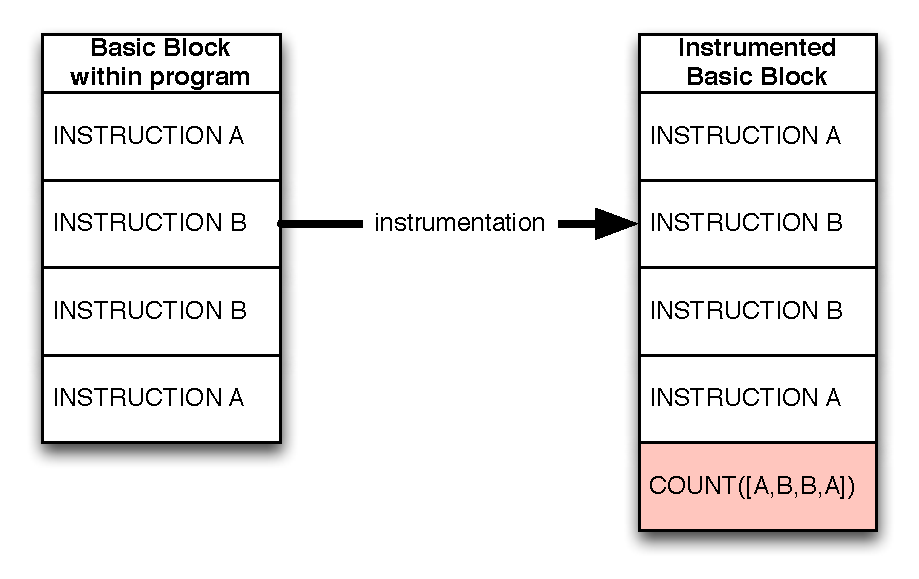
\includegraphics[width=0.4\textwidth]{instructionbitcode}
\caption{bitcode instrumentation}
\end{figure}

\subsection{Physical Implementation Description}

Functions shown on algorithm 2 are written in C++, compiled separately and then linked to the input program later (as described in the instructions), but calls to these functions have to be inserted using the \code{opt} pass.

Again, we used the \code{ModulePass} class and \code{RunOnModule(Module \&M)} method for the implementation. First, we iterate through each basic block (using the \code{Module} and \code{Function} iterators) and collect the instructions for that block using the \code{CI.getOpcodeName()} method provided by the LLVM library for each instruction \code{CI}. We then concatenate all of these instructions into some comma separated string called \code{result}. Finally, we use the following code snippet to call the linked function :

\begin{frame}[fragile]
%\frametitle{Inserting source code}
\lstset{language=C++,
                basicstyle=\ttfamily,
                keywordstyle=\color{blue}\ttfamily,
                stringstyle=\color{red}\ttfamily,
                commentstyle=\color{cool}\ttfamily,
                morecomment=[l][\color{magenta}]{\#}
}
\begin{lstlisting}
// BE points to the end of the BB
builder.SetInsertPoint(BB,BE);
Value* myStr = 
builder.CreateGlobalStringPtr(result);
builder.CreateCall(hookCount,myStr);
\end{lstlisting}
\end{frame}
As can be seen from this snippet, we used an \code{IRBuilder} class to help constructing the call insertion. We did not have to concatenate instructions (we could have used an array of strings), but strings are easier to pass to call instructions using the LLVM library than arrays of strings. Notice that the C++ implementation of the \code{count} function accepts a \code{char*} as input, accordingly.

\subsection{Benchmark Analysis}

In the execution of the gcd example, the main function calls the \code{gcd()} function on input \code{(72,32)}. We can easily predict that the \code{gcd} will be called twice recursively before returning to main, which in turn will return at the end of execution. No other function calls are made. As such we should expect the \code{ret} instruction to be called 4 times, which is precisely the number of times it is called in the benchmark we generated.

\section{Profiling branch bias}
We wish to measure the branch bias on each function of our program. As for the previous section, this type of information can only be collected at run-time and requires instrumentation of the bytecode.

%The project was completed succesfully . Learning outcomes were a working understanding of LLVM optimiser passes. We are capable of transforming and instrumenting code. We have developed an efficient method to develop, test and debug the LLVM source tree with a debug api and symbol indexed code base via the eclipse CDT. Understanding how to instrument code has provided a powerful tool for analysis of any optimisation heuristics applied by other opt passes. Instrumentation will allow us to both formulate and test heuristics based on the performance of compiled code.\\
To conclude, this project has provided us with a solid foundation for the second upcoming project for CSE 231

%{\footnotesize \bibliographystyle{acm}
%\bibliography{sample.bib}}
%\theendnotes
\end{document}







